\documentclass[xetex,mathserif,serif]{beamer}

\usepackage{xunicode}
\usepackage{xltxtra}
\usepackage{color}
\usepackage{url}
\usepackage{listings}
\usepackage{fontspec}
\usepackage{geometry}
\usepackage{lastpage}
\usepackage{fancyhdr}
\usepackage{amsmath}
\usepackage{amsthm}
\usepackage{amssymb}
\usepackage{blkarray}
\usepackage{multicol}
\usepackage{relsize}

\definecolor{solarized@base03}{HTML}{002B36}
\definecolor{solarized@base02}{HTML}{073642}
\definecolor{solarized@base01}{HTML}{586e75}
\definecolor{solarized@base00}{HTML}{657b83}
\definecolor{solarized@base0}{HTML}{839496}
\definecolor{solarized@base1}{HTML}{93a1a1}
\definecolor{solarized@base2}{HTML}{EEE8D5}
\definecolor{solarized@base3}{HTML}{FDF6E3}
\definecolor{solarized@yellow}{HTML}{B58900}
\definecolor{solarized@orange}{HTML}{CB4B16}
\definecolor{solarized@red}{HTML}{DC322F}
\definecolor{solarized@magenta}{HTML}{D33682}
\definecolor{solarized@violet}{HTML}{6C71C4}
\definecolor{solarized@blue}{HTML}{268BD2}
\definecolor{solarized@cyan}{HTML}{2AA198}
\definecolor{solarized@green}{HTML}{859900}
\definecolor{yaleblue}{HTML}{0E4C92}

\setbeamertemplate{navigation symbols}{}
% \setbeamerfont{title}{family=\old}
% \setbeamerfont{author}{family=\tfont}%
% \setbeamerfont{frametitle}{family=\oldA}
% \setbeamerfont{date}{family=\dfont}

\setbeamertemplate{itemize items}{--}
\setbeamercolor*{item}{fg=black}

\defaultfontfeatures{Mapping=tex-text}
\hypersetup{pdfstartview={FitH}}

\newcommand{\old}[1]{\fontspec[Alternate=1,Ligatures={Common}]{Hoefler Text}\fontsize{18pt}{30pt}\selectfont #1}%
\newcommand{\oldA}[1]{\fontspec[Alternate=1,Ligatures={Common, Rare}]{Hoefler Text}\fontsize{12pt}{15pt}\selectfont #1}%
\newcommand{\oldB}[1]{\fontspec[Ligatures={Common}]{Didot}\fontsize{12pt}{15pt}\color{solarized@base02}\selectfont #1}%
\newcommand{\tfont}[1]{\fontspec[Alternate=1,Ligatures={Common}]{Hoefler Text}\fontsize{12pt}{20pt}\selectfont #1}%
\newcommand{\dfont}[1]{\fontspec[Ligatures={Common}]{Didot}\fontsize{12pt}{12pt}\selectfont #1}%

\newcommand{\minimize}{\mathop{\mathrm{minimize}}}
\newcommand{\argmin}{\mathop{\mathrm{arg\,min}}}
\newcommand{\argmax}{\mathop{\mathrm{arg\,max}}}
\newcommand{\st}{\mathop{\mathrm{subject\,\,to}}}

\newcommand\independent{\protect\mathpalette{\protect\independenT}{\perp}}
\def\independenT#1#2{\mathrel{\rlap{$#1#2$}\mkern2mu{#1#2}}}

\setlength{\parindent}{0pt}
\setlength{\parskip}{12pt}

\setromanfont [Ligatures={Common}, Numbers={OldStyle}, Variant=01,
 BoldFont={LinLibertine_RB.otf},
 ItalicFont={LinLibertine_RI.otf},
 BoldItalicFont={LinLibertine_RBI.otf}
 ]{LinLibertine_R.otf}



\begin{document}

%%%%%%%%%%%%%%%%%%%%%%%%%%%%%%%%%%%%%%%%%%%%%%%%%%%
\begin{frame}[fragile] \frametitle{}

\vfill

{\fontsize{0.7cm}{0cm}\selectfont Lecture 23 \\\vspace{0.2cm}
Alternating Direction Method of Multipliers}\\\vspace{0.5cm}
09 December 2015

\vspace{2cm}

\begin{minipage}{0.6\textwidth}
Taylor B. Arnold \\
Yale Statistics  \\
STAT 312/612
\end{minipage}
\hfill
\begin{minipage}{0.3\textwidth}\raggedleft

\includegraphics[scale=0.3]{../yale-logo.png}
\end{minipage}%

\end{frame}

%%%%%%%%%%%%%%%%%%%%%%%%%%%%%%%%%%%%%%%%%%%%%%%%%%%
\begin{frame}[fragile] \frametitle{}

{\color{yaleblue}\fontsize{16pt}{20pt}\selectfont Class Notes}

\begin{itemize}
\item Problem Set 7 - Available now, hand in at 24 Hillhouse by 4pm on December 16th
\end{itemize}

\end{frame}

%%%%%%%%%%%%%%%%%%%%%%%%%%%%%%%%%%%%%%%%%%%%%%%%%%%
\begin{frame}[fragile] \frametitle{}

{\color{yaleblue}\fontsize{16pt}{20pt}\selectfont Midterm II}

Easy solution to question 1:
\begin{verbatim}
> X <- matrix(rnorm(12),nrow=4)
> s <- svd(X)
> svals <- c(1,1,1e-10)
> X <- s$u %*% diag(svals) %*% t(s$v)
> X
           [,1]        [,2]      [,3]
[1,] -0.3425962  0.50634449 0.1048543
[2,]  0.2080486 -0.53566801 0.3398572
[3,] -0.3472912  0.07954308 0.8733534
[4,]  0.2120066 -0.45074100 0.1781087
\end{verbatim}

\end{frame}

%%%%%%%%%%%%%%%%%%%%%%%%%%%%%%%%%%%%%%%%%%%%%%%%%%%
\begin{frame}[fragile] \frametitle{}

Now notice that a direct solve does not work well:
\begin{verbatim}
> beta <- c(1,1,1)
> y <- X %*% beta
> solve(t(X) %*% X, t(X) %*% y, tol=0)
            [,1]
[1,] -0.62017237
[2,]  0.01868727
[3,]  0.44511010
\end{verbatim}

\end{frame}

%%%%%%%%%%%%%%%%%%%%%%%%%%%%%%%%%%%%%%%%%%%%%%%%%%%
\begin{frame}[fragile] \frametitle{}

But the pseudo inverse does:
\begin{verbatim}
> pseudo <- s$v %*% diag(1/svals) %*% t(s$u)
> pseudo %*% y
         [,1]
[1,] 1.000001
[2,] 1.000001
[3,] 1.000000
\end{verbatim}

\end{frame}



%%%%%%%%%%%%%%%%%%%%%%%%%%%%%%%%%%%%%%%%%%%%%%%%%%%
\begin{frame}[fragile] \frametitle{}

\begin{center}
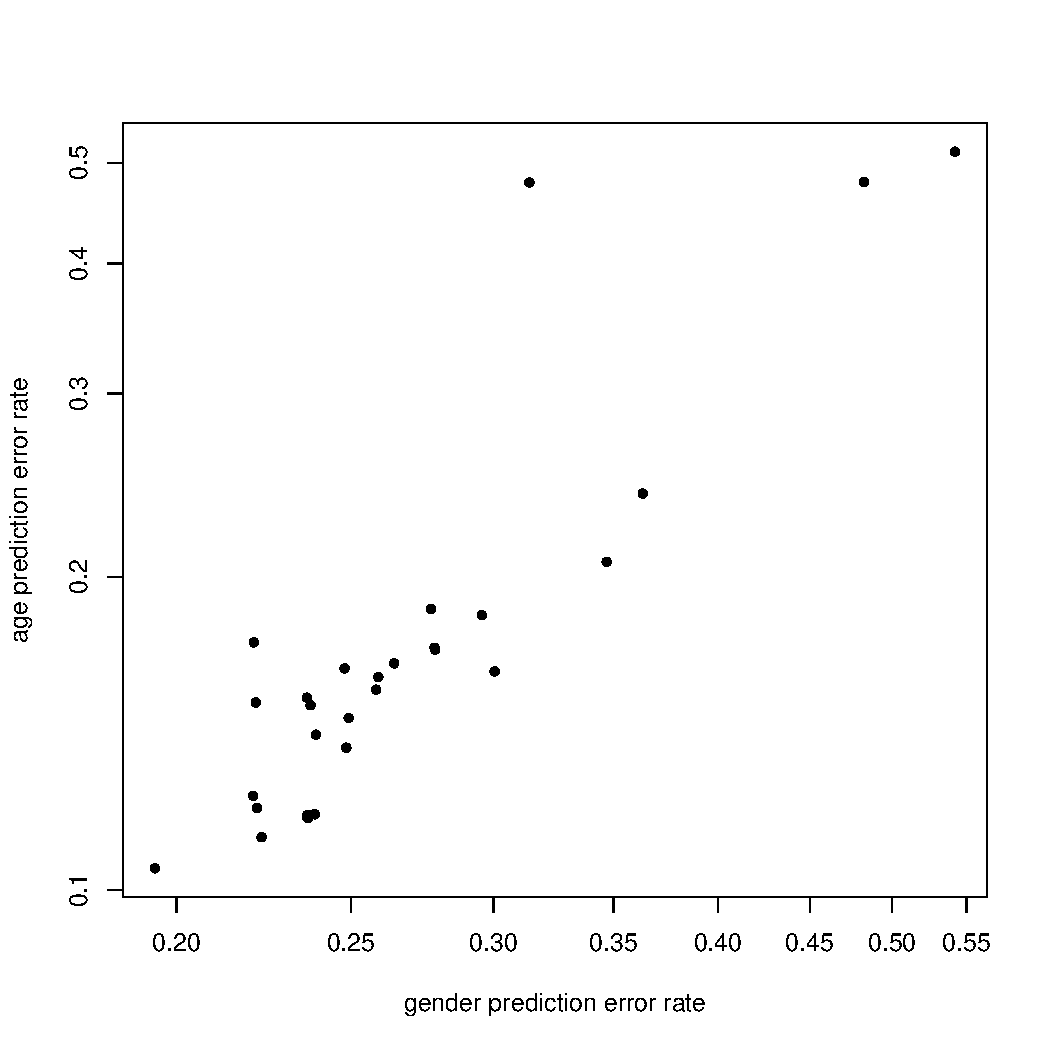
\includegraphics[height=\textheight]{img/predFig.pdf}
\end{center}

\end{frame}

%%%%%%%%%%%%%%%%%%%%%%%%%%%%%%%%%%%%%%%%%%%%%%%%%%%
\begin{frame}[fragile] \frametitle{}

\begin{flushright}
{\color{yaleblue}\sc\fontsize{1cm}{0cm}\selectfont ADMM}
\end{flushright}

\end{frame}


%%%%%%%%%%%%%%%%%%%%%%%%%%%%%%%%%%%%%%%%%%%%%%%%%%%
\begin{frame}[fragile] \frametitle{}

Consider the following minimization problem:
\begin{align*}
\begin{array}{ll}
\text{minimize} & f(x) \\
\text{subject to} & Ax = b
\end{array}
\end{align*}
\pause The Lagrangian function is defined as:
\begin{align*}
L(x,y) &= f(x) + y^t (Ax - b)
\end{align*}

\end{frame}

%%%%%%%%%%%%%%%%%%%%%%%%%%%%%%%%%%%%%%%%%%%%%%%%%%%
\begin{frame}[fragile] \frametitle{}

As described last time, the dual function is defined as:
\begin{align*}
g(y) &= \inf_x L(x,y)
\end{align*}
And the corresponding dual problem is:
\begin{align*}
y^{*} &= \argmax_y g(y)
\end{align*}
Which yields the solution $x^{*}$:
\begin{align*}
x^{*} &= \argmin_x L(x, y^{*})
\end{align*}
With most of the work occurring in solving the dual problem.

\end{frame}

%%%%%%%%%%%%%%%%%%%%%%%%%%%%%%%%%%%%%%%%%%%%%%%%%%%
\begin{frame}[fragile] \frametitle{}

If we have an analytic form of the function $g$ and its gradient,
gradient ascent can be used to repeatedly update $y$ until convergence
by:
\begin{align*}
y^{k+1} &= y^{k} + \alpha \cdot \nabla g (y^k)
\end{align*}
\pause Likewise, dual ascent is given by:
\begin{align*}
x^{k+1} &= \argmin_x L(x, y^k) \\
y^{k+1} &= y^{k} + \alpha \cdot (A x^{k+1} - b)
\end{align*}
Which converges to the correct solution under strong assumptions.

\end{frame}

%%%%%%%%%%%%%%%%%%%%%%%%%%%%%%%%%%%%%%%%%%%%%%%%%%%
\begin{frame}[fragile] \frametitle{}

Now, consider if $f$ can be separated as follows:
\begin{align*}
f(x) &= \sum_i f_i (x_i)
\end{align*}
The Lagrangian can the be written as:
\begin{align*}
L(x,y) &= \sum_i L_i (x_i, y) \\
&= \sum_i f_i(x) + y^t A_i x_i - y^t b
\end{align*}
And therefore the $x$-step in dual ascent can be parallelized over each
$x_i$.

\end{frame}

%%%%%%%%%%%%%%%%%%%%%%%%%%%%%%%%%%%%%%%%%%%%%%%%%%%
\begin{frame}[fragile] \frametitle{}

Specifically:
\begin{align*}
x^{k+1}_i &= \argmin_{x_i} L_i(x_i, y^k) \\
y^{k+1} &= y^{k} + \alpha \cdot (A x^{k+1} - b)
\end{align*}
Which again, converges to the correct solution under strong assumptions.

\end{frame}

%%%%%%%%%%%%%%%%%%%%%%%%%%%%%%%%%%%%%%%%%%%%%%%%%%%
\begin{frame}[fragile] \frametitle{}

Now, consider the augmented Lagrangian:
\begin{align*}
L_\rho (x, y) &= f(x) + y^t (Ax - b) + \left(\rho / 2\right)|| Ax - b ||_2^2
\end{align*}
For some value of $\rho > 0$. This makes dual ascent far more robust, and yields
the following updates:
\begin{align*}
x^{k+1} &= \argmin_x L_\rho (x, y^{k}) \\
y^{k+1} &= y^k + \rho (A x^{k+1} - b)
\end{align*}
Notice that the $\alpha$ in the $y$-step has been replaced by the $\rho$
in the augmented Lagrangian. This is called the \textbf{method of multipliers}.

\end{frame}

%%%%%%%%%%%%%%%%%%%%%%%%%%%%%%%%%%%%%%%%%%%%%%%%%%%
\begin{frame}[fragile] \frametitle{}

The method of multipliers will converge under much more relaxed conditions, but
we have a squared norm of the penalty this will no longer allow for splitting the
optimization problem across $f_i(x_i)$'s.

\end{frame}

%%%%%%%%%%%%%%%%%%%%%%%%%%%%%%%%%%%%%%%%%%%%%%%%%%%
\begin{frame}[fragile] \frametitle{}

The method \textbf{alternating direction method of multipliers}, or \text{ADMM},
combines the splitting capability of dual ascent with the robustness
of the method of multipliers. It solves the optimization problem:
\begin{align*}
\begin{array}{ll}
\text{minimize} & f(x) + g(z) \\
\text{subject to} & Ax + Bz = c
\end{array}
\end{align*}
With the augmented Lagrangian:
\begin{align*}
L_\rho (x, z, y) &= f(x) + g(z) + y^t (Ax + Bz - c) + \left(\rho / 2\right)|| Ax + Bz - c ||_2^2
\end{align*}

\end{frame}

%%%%%%%%%%%%%%%%%%%%%%%%%%%%%%%%%%%%%%%%%%%%%%%%%%%
\begin{frame}[fragile] \frametitle{}

To solve this, we add three types of updates:
\begin{align*}
x^{k+1} &= \argmin_x L_\rho (x, z^k, y^k) \\
z^{k+1} &= \argmin_z L_\rho (x^{k+1}, z, y^k) \\
y^{k+1} &= y^{k} + \rho \cdot (A x^{k+1} + B z^{k+1} - c)
\end{align*}
Where solving the first two steps simultaneously would yield the
same solution as the method of multipliers. The \textit{alternating}
in the name refers to alternating between $x$-updates and $z$-updates.

\end{frame}

%%%%%%%%%%%%%%%%%%%%%%%%%%%%%%%%%%%%%%%%%%%%%%%%%%%
\begin{frame}[fragile] \frametitle{}

If we replace $u_k = (1/\rho) y^k$, this allows combining the linear and
quadratic terms in the augmented Lagrangian. The update now can be written
explicitly:
\begin{align*}
x^{k+1} &= \argmin_x \left\{ f(x) + (\rho / 2) || A x + B z^{k} - c + u^k ||_2^2 \right\} \\
z^{k+1} &= \argmin_z \left\{ f(x) + (\rho / 2) || A x^{k+1} + B z - c + u^k ||_2^2 \right\} \\
u^{k+1} &= u^{k} + (A x^{k+1} + B z^{k+1} - c)
\end{align*}

\end{frame}

%%%%%%%%%%%%%%%%%%%%%%%%%%%%%%%%%%%%%%%%%%%%%%%%%%%
\begin{frame}[fragile] \frametitle{}

Assume $f$ and $g$ are convex, closed, and proper and $L_0$ has
a saddle point. Then ADMM converges in both feasibility (does the
constraint hold) and optimality (is the function to be optimized near
its optimal value).

\end{frame}

%%%%%%%%%%%%%%%%%%%%%%%%%%%%%%%%%%%%%%%%%%%%%%%%%%%
\begin{frame}[fragile] \frametitle{}

Consider now the lasso problem. We'll write it here in `numerical analysis'
notation (so $A$ is the data matrix, $x$ in the unknown parameter, and $b$ is
the response):
\begin{align*}
\argmin_x (1/2) || A x - b ||_2^2 + \lambda || x ||_1
\end{align*}
As we did last class, we'll write this as a a constrained problem:
\begin{align*}
\begin{array}{ll}
\text{minimize} & (1/2) || A x - b ||_2^2 + \lambda || z ||_1 \\
\text{subject to} & x - z = 0
\end{array}
\end{align*}
Where we have separated the $\ell_2$-loss as a function of $x$ and the
$\ell_1$-penalty as a function of $z$.

\end{frame}

%%%%%%%%%%%%%%%%%%%%%%%%%%%%%%%%%%%%%%%%%%%%%%%%%%%
\begin{frame}[fragile] \frametitle{}

So the $x$-step in ADMM amounts to finding the minimum over $x$
of the following quantity:
\begin{align*}
f(x) + (\rho / 2) || Ax + Bz - c + u ||_2^2
&= ||A x - b ||_2^2 + (\rho / 2) || x - z + u ||_2^2 \\
\end{align*}
\pause If we translate to $w = x - z + u$ this is just ridge regression
on $w$, which we have an analytic formula for. Transforming the variables
we get specifically:
\begin{align*}
x^{k+1} &= (A^t A + \rho I)^{-1}  (A^t b + \rho z^k - u^k)
\end{align*}

\end{frame}


%%%%%%%%%%%%%%%%%%%%%%%%%%%%%%%%%%%%%%%%%%%%%%%%%%%
\begin{frame}[fragile] \frametitle{}

Now, the $z$-step in ADMM amounts to finding the minimum over $x$
\begin{align*}
g(z) + (\rho / 2) || Ax + Bz - c + u ||_2^2
&= \lambda || z ||_1 + (\rho / 2) || x - z + u ||_2^2 \\
\end{align*}
And dividing by $\rho$ gives:
\begin{align*}
\argmin_z \left\{ (1 / 2) || (x + u) - z ||_2^2 + \lambda / \rho || z ||_1 \right\} \\
\end{align*}
Which is just the lasso without an $X$ matrix and on the response $x + u$.

\end{frame}

%%%%%%%%%%%%%%%%%%%%%%%%%%%%%%%%%%%%%%%%%%%%%%%%%%%
\begin{frame}[fragile] \frametitle{}

From lecture 17, we have an analytic formula for the simple lasso case
where the variables are uncorrelated. Here we have an even more easy
formula because $X$ is the identity itself.

\pause Specifically, we have the following formula for the lasso regression
\begin{align*}
z^{k+1}_i &= \left\{ \begin{array}{ll}
x_i + u_i - \lambda / \rho &\, (x_i + u_i) \geq \lambda / \rho \\
x_i + u_i + \lambda / \rho &\, (x_i + u_i) \leq -\lambda / \rho \\
0 &\, \text{else} \\
\end{array} \right.
\end{align*}
Called soft-thresholding and denoted by (for the penalty $\lambda / \rho$):
\begin{align*}
z^{k+1} &= S_{\lambda / \rho} (x_i + u_i)
\end{align*}

\end{frame}

%%%%%%%%%%%%%%%%%%%%%%%%%%%%%%%%%%%%%%%%%%%%%%%%%%%
\begin{frame}[fragile] \frametitle{}

So the full ADMM lasso update is given by:
\begin{align*}
x^{k+1} &= (A^t A + \rho I)^{-1}  (A^t b + \rho z^k - y^k) \\
z^{k+1}_i &= S_{\lambda / \rho} (x_i + u_i) \\
u^{k+1} &= u^k + \rho (x^{k+1} - z^{k+1})
\end{align*}
Or, in other words, we iteratively do ridge regression followed by
soft-thresholding.

\pause The hard computational part is take the SVD of $A$, which only
needs to be done once, in order to get the first $x$-update. There are
many ways of doing this in parallel, particularly when $n > p$. Otherwise,
all of these ADMM steps can be solved locally on the data. This allows
for massive parallelization gains.

\end{frame}

%%%%%%%%%%%%%%%%%%%%%%%%%%%%%%%%%%%%%%%%%%%%%%%%%%%
\begin{frame}

\begin{center}
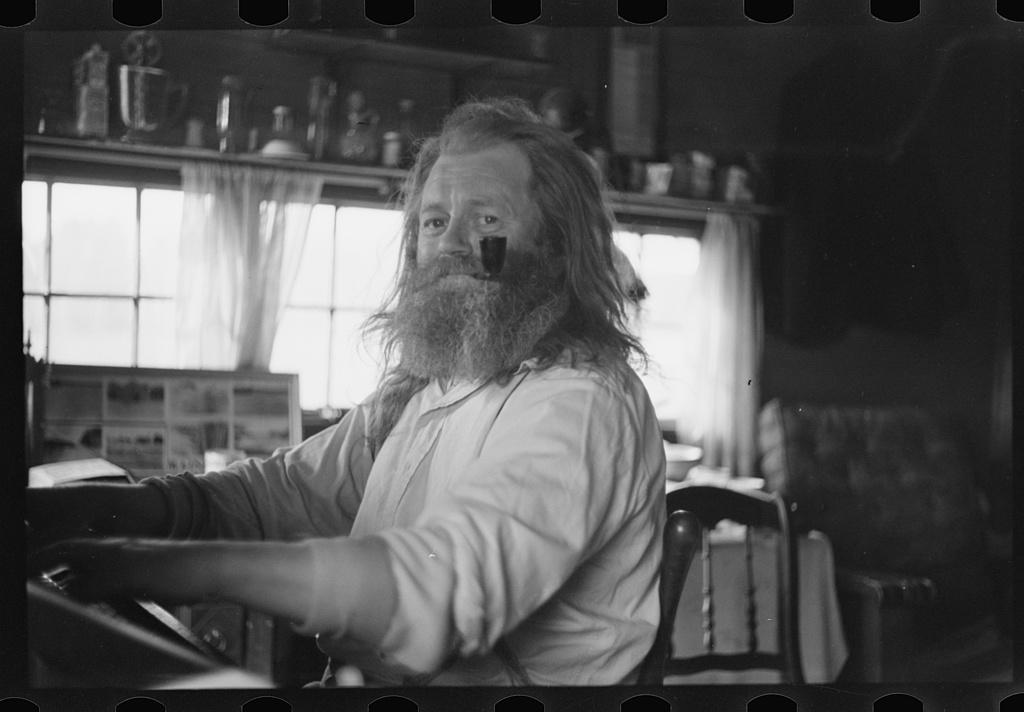
\includegraphics[width=\textwidth]{img/img0.jpg}
\end{center}

\end{frame}

%%%%%%%%%%%%%%%%%%%%%%%%%%%%%%%%%%%%%%%%%%%%%%%%%%%
\begin{frame}

\begin{center}

\includegraphics[width=\textwidth]{img/img1.jpg}
\end{center}

\end{frame}


%%%%%%%%%%%%%%%%%%%%%%%%%%%%%%%%%%%%%%%%%%%%%%%%%%%
\begin{frame}

\begin{center}
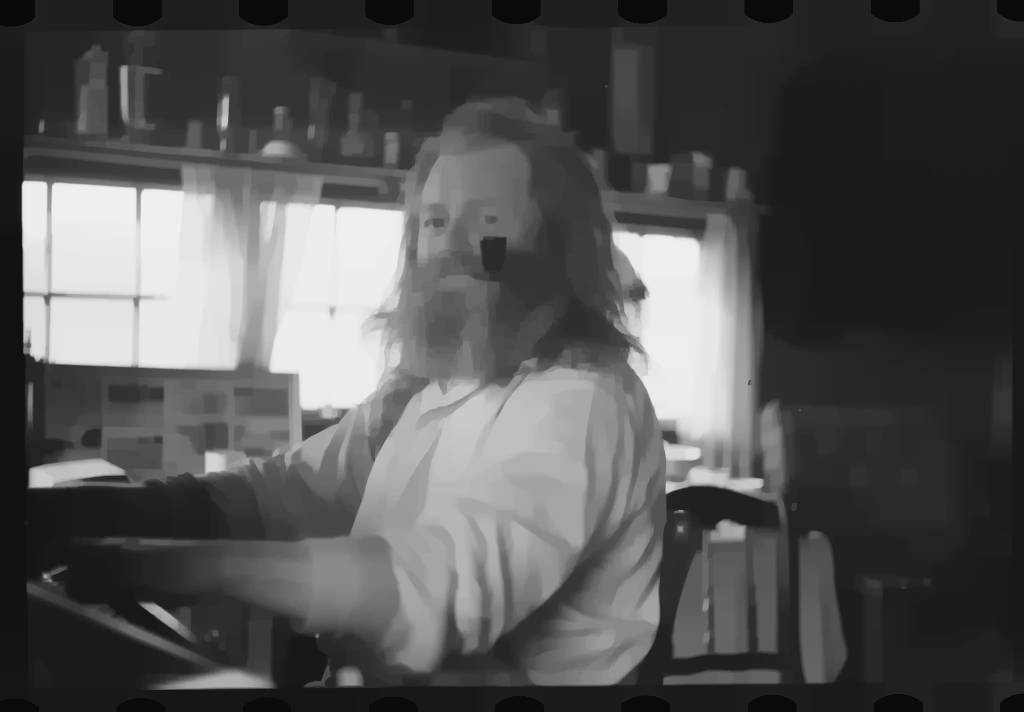
\includegraphics[width=\textwidth]{img/img2.jpg}
\end{center}

\end{frame}

%%%%%%%%%%%%%%%%%%%%%%%%%%%%%%%%%%%%%%%%%%%%%%%%%%%
\begin{frame}

\begin{center}
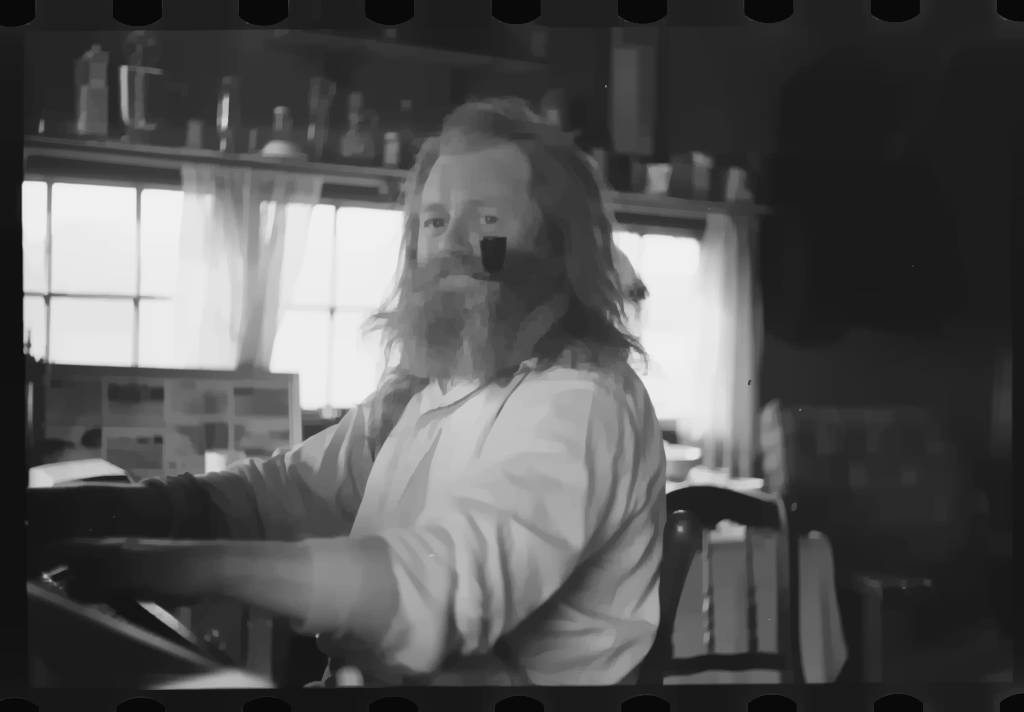
\includegraphics[width=\textwidth]{img/img3.jpg}
\end{center}

\end{frame}

%%%%%%%%%%%%%%%%%%%%%%%%%%%%%%%%%%%%%%%%%%%%%%%%%%%
\begin{frame}[fragile] \frametitle{}

\begin{flushright}
{\color{yaleblue}\sc\fontsize{1cm}{0cm}\selectfont Closing thoughts / summary}
\end{flushright}

\end{frame}

%%%%%%%%%%%%%%%%%%%%%%%%%%%%%%%%%%%%%%%%%%%%%%%%%%%
\begin{frame}[fragile] \frametitle{}

In the first lecture I said:
\begin{quote}
Linear Models is both a capstone to the 241/242 sequence
and the breadth to compliment 610's depth. It also
serves as a link between the statistical inference courses
and the applied data analysis courses.

\medskip

Topics will be oriented around linear models (obviously) but
the course is somewhat of a hodgepodge of topics and applications.
\end{quote}
I think this has been generally true; hopefully it has been both
a \magenta{useful} and \cyan{interesting} hodgepodge of topics.

\end{frame}

%%%%%%%%%%%%%%%%%%%%%%%%%%%%%%%%%%%%%%%%%%%%%%%%%%%
\begin{frame}[fragile] \frametitle{}

\textbf{Techniques}
\begin{enumerate}
\item classical linear regression
\item weighted least squares
\item hierarchical linear models
\item logistic regression
\item singular value decomposition
\item ridge regression
\item principal components
\item lasso regression
\item elastic net
\item generalized lasso regression
\end{enumerate}

\end{frame}

%%%%%%%%%%%%%%%%%%%%%%%%%%%%%%%%%%%%%%%%%%%%%%%%%%%
\begin{frame}[fragile] \frametitle{}

\textbf{Applications}
\begin{enumerate}
\item historical data from 1890's (Galton's experiments)
\item larger datasets (airline)
\item unstructured dataset (image corpus, text corpus)
\end{enumerate}

\end{frame}

%%%%%%%%%%%%%%%%%%%%%%%%%%%%%%%%%%%%%%%%%%%%%%%%%%%
\begin{frame}[fragile] \frametitle{}

\textbf{Numerical algorithms}
\begin{enumerate}
\item Cholesky w/ backsolve and forwardsolve for LS problem
\item QR of X trick for LS
\item pseudoinverse trick for LS
\item Newton-Raphson, iteratively reweighted least squares (glm)
\item LARs, homotopy path solution for solving lasso
\item coordinate descent (elastic net, problem set 7)
\item Lagrangian dual problem (generalized lasso)
\item alternating direction method of multipliers (today, lasso)
\end{enumerate}

\end{frame}

%%%%%%%%%%%%%%%%%%%%%%%%%%%%%%%%%%%%%%%%%%%%%%%%%%%
\begin{frame}[fragile] \frametitle{}

If you enjoyed this, consider taking \textbf{\cyan{Data Mining and Machine Learning (STAT 365/665)}}
with me in the Spring. It will have an even
heavier focus on applications with considerably less theory.

\end{frame}

\end{document}











